% arXiv/pdfLaTeX requirement
\pdfoutput=1

\documentclass[11pt]{article}
\usepackage[review]{acl}
\usepackage{times}
\usepackage{latexsym}
\usepackage[T1]{fontenc}
\usepackage[utf8]{inputenc}
\usepackage{microtype}
\usepackage{inconsolata}
\usepackage{graphicx}
\usepackage{booktabs}
\usepackage{amsmath}
\usepackage{amssymb}
\usepackage{enumitem}
\usepackage{multirow}
\usepackage{tikz}
\usepackage{pgfplots}
\pgfplotsset{compat=1.18}

\definecolor{grpocol}{RGB}{70,130,180}
\definecolor{hcpccol}{RGB}{210,70,70}
\definecolor{nsrcol}{RGB}{50,155,70}

\newcommand\blfootnote[1]{%
  \begingroup
  \renewcommand\thefootnote{}\footnote{#1}%
  \addtocounter{footnote}{-1}%
  \endgroup
}

\newcommand{\hcpc}{\textsc{HCPC}}
\newcommand{\rlvr}{\textsc{RLVR}}
\newcommand{\grpo}{\textsc{GRPO}}
\newcommand{\nsr}{\textsc{NSR}}

\title{Cross-Rollout Consistency and Negative Sample Rewards\\
       for Chart Question Answering}

\author{Sumaiya Ahmed$^{*}$, Nafisa Haque$^{*}$, Jannatul Fardus Rakhi$^{*}$ \\
  \\
  Department of Computer Science and Engineering \\
  Islamic University of Technology, Dhaka, Bangladesh \\
  \texttt{\{sumaiya210041223, nafisa210041231, rakhi210041237\}@iut-dhaka.edu}}

\begin{document}
\maketitle

%------------------------------------------------------------------
\begin{abstract}
\blfootnote{$^*$Equal Contribution}
Chart question answering (ChartQA) demands sequential success at chart-type
identification, data-table extraction, and verifiable reasoning---yet current
reinforcement learning with verifiable rewards (\rlvr) treats each sampled
rollout independently, discarding the cross-rollout structure of jointly
generated outputs.
We propose \textbf{Hierarchical Correct-Path Consistency (\hcpc)}, a group-level
bonus applied exclusively to fully-correct rollouts that simultaneously rewards
type consistency ($C_\text{type}$), table consistency ($C_\text{table}$), and
per-rollout reasoning uniqueness ($D_\text{reason}$).
We also conduct the first evaluation of Negative Sample Reward (\nsr) on a
vision-language model (VLM), extending negative-only policy updates from text
mathematics to structured visual reasoning.
Experiments on ChartQA and ChartFC with Qwen2.5-VL-3B-Instruct show that
\nsr{} outperforms \grpo{} by 0.4~pp on in-domain pass@1 and 7.0~pp on
out-of-distribution pass@1. \hcpc{} achieves the best pass@4 ($+$1.2~pp) but
causes severe format collapse on fact-checking inputs (compliance 0.664 vs.\ 0.988
for \grpo). We diagnose three root causes and provide concrete reward-design
guidance.
\end{abstract}

%==================================================================
\section{Introduction}

Chart question answering is a structured visual reasoning task in which a model
must identify the chart type, reconstruct a data table from a chart image, and
apply numerical or logical operations over that table to produce a verifiable
answer.
Errors at any stage propagate forward: an incorrect table makes correct arithmetic
impossible, while a malformed output prevents automated evaluation entirely.
\rlvr{} has emerged as a promising approach for this task, replacing costly
annotated reasoning demonstrations with lightweight rule-based reward
signals~\citep{sinha2025chartrvr}.
However, standard \rlvr{} methods such as \grpo{}~\citep{shao2024deepseekmath}
evaluate each of the $K$ sampled rollouts independently, discarding an important
structural property: jointly-sampled rollouts provide cross-rollout evidence about
perceptual stability and reasoning diversity that per-rollout rewards cannot
capture.

We address this with \textbf{Hierarchical Correct-Path Consistency (\hcpc)}, a
cross-rollout bonus applied to rollouts that simultaneously satisfy chart-type,
table, and answer correctness.
Within this correct pool, \hcpc{} rewards type-identification agreement
($C_\text{type}$), pairwise table-extraction similarity ($C_\text{table}$), and
reasoning-path uniqueness, assigning higher rewards to correct rollouts whose
reasoning most differs from their peers.
The inductive bias is deliberate: perceptual interpretation should be stable while
valid reasoning paths should remain diverse.

Separately, we evaluate \textbf{Negative Sample Reward (\nsr)}~\citep{zhu2025nsr}
on a VLM for the first time.
\nsr{} applies zero gradient to correct rollouts and a penalty to incorrect ones,
preserving the model's distribution over valid strategies without explicit
diversity engineering.
Our experiments show that \nsr{} achieves the best pass@1 on both benchmarks,
with its 7.0~pp out-of-distribution (OOD) advantage on ChartFC attributable to
distribution preservation.
\hcpc{} expands the reachable solution set (best pass@4) but suffers from three
diagnosable failure modes: reasoning diversity is structurally capped at 3B-parameter
scale regardless of the incentive applied; the cross-rollout bonus fires only when
$|\mathcal{F}| \ge 2$, concentrating signal on easy samples; and the absence of a
format gate on fact-checking inputs allows format-free responses to contaminate the
correct pool.

%==================================================================
\section{Related Work}

\paragraph{Chart QA benchmarks.}
ChartQA~\citep{masry2022chartqa} provides diverse chart-image questions spanning
numeric computation, boolean comparison, string identification, and multi-hop
reasoning, with relaxed numeric matching to account for axis-reading ambiguity.
ChartFC~\citep{akhtar2023chartfc} reframes chart understanding as binary
fact-checking; ground-truth data tables are absent, making it a natural OOD
benchmark for models trained on numeric QA.
PlotQA~\citep{plotqa} covers scientific plots with complex aggregation queries.

\paragraph{RLVR for chart reasoning.}
\citet{sinha2025chartrvr} introduced \grpo-based \rlvr{} with rule-based rewards
for chart-type, table, and process conformity, showing that objective reward checks
outperform annotated reasoning demonstrations on ChartQA.
Chart-R1~\citep{chart_r1} and BIGCHARTS-R1~\citep{bigcharts} extended this with
chain-of-thought supervision and larger-scale visual fine-tuning.

\paragraph{Diversity-preserving policy updates.}
\citet{zhu2025nsr} decomposed \rlvr{} into positive sample reinforcement (PSR)
and negative sample reinforcement (\nsr), showing that \nsr{} alone matches or
surpasses \grpo{} and PPO on mathematical reasoning benchmarks.
Their evaluation was restricted to text-only models; this work extends \nsr{} to
a VLM setting with multi-component, noisy rewards.
\citet{yu2025dapo} proposed a weighted hybrid ($\lambda$-PSR $+$ \nsr) that
achieved further improvements on text-based tasks.

%==================================================================
\section{Method}\label{sec:method}

\paragraph{Task setup and base reward.}
Given chart image $I$ and question $Q$, the model samples $K = 4$ rollouts at
temperature 0.8.
Each rollout $y_i$ is parsed into chart type $\hat{\tau}_i$, data table
$\hat{\mathcal{T}}_i$, reasoning trace $\hat{r}_i$, and final answer $\hat{a}_i$.
The base reward $R_i^{\text{base}}$ follows~\citet{sinha2025chartrvr}: format
compliance (0--2), answer accuracy (0--1), output length (0--2), tag count (0--2),
chart-type match (0--1), and table structure (0--2).
The total reward is $R_i = R_i^{\text{base}} + R_i^{\hcpc}$.

\paragraph{HCPC correct pool.}
\hcpc{} conditions exclusively on fully-correct rollouts:
%
\begin{equation}
  \mathcal{F} = \bigl\{\, i \;\big|\;
    \hat{\tau}_i = \tau^*,\;\;
    \operatorname{sim}(\hat{\mathcal{T}}_i,\, \mathcal{T}^*) \ge \delta,\;\;
    \hat{a}_i \approx a^*
  \,\bigr\}
  \label{eq:filter}
\end{equation}
%
with threshold $\delta = 0.6$.
Before Eq.~(\ref{eq:filter}), format compliance is enforced: a rollout must
have well-formed XML structure and a valid JSON table schema to be eligible.
This gate prevents format-free responses from contaminating the correct pool.
If $|\mathcal{F}| < 2$, \hcpc{} returns zero for all rollouts.

\paragraph{Consistency and diversity terms.}
Three cross-rollout metrics are computed over $\mathcal{F}$:
%
\begin{equation}
\begin{aligned}
  C_\text{type}  &= \frac{
    \max_{\tau}\;\bigl|\{i \in \mathcal{F} : \hat{\tau}_i = \tau\}\bigr|
  }{|\mathcal{F}|} \\[6pt]
  C_\text{table} &= \frac{2}{|\mathcal{F}|(|\mathcal{F}|-1)}
                    \sum_{\substack{i < j \\ i,j \in \mathcal{F}}}
                    \operatorname{sim}\!\bigl(\hat{\mathcal{T}}_i,\, \hat{\mathcal{T}}_j\bigr)
\end{aligned}
\label{eq:consistency}
\end{equation}
%
\begin{equation}
  D_\text{reason} = 1 - \frac{2}{|\mathcal{F}|(|\mathcal{F}|-1)}
    \sum_{\substack{i < j \\ i,j \in \mathcal{F}}}
    \cos\!\bigl(\mathbf{e}_i,\, \mathbf{e}_j\bigr)
  \label{eq:diversity}
\end{equation}
%
where $\mathbf{e}_i = \operatorname{enc}(\hat{r}_i)$ is the sentence embedding of
reasoning trace $\hat{r}_i$ via \texttt{all-MiniLM-L6-v2}~\citep{reimers2019sbert}.

\paragraph{Per-rollout differentiated reward.}
Rather than assigning a uniform group bonus, each correct rollout $k$ receives a
reward based on its uniqueness relative to its peers in $\mathcal{F}$:
%
\begin{equation}
\begin{aligned}
  u_k &= 1 - \frac{1}{|\mathcal{F}|-1}
             \sum_{\substack{j \in \mathcal{F} \\ j \neq k}}
             \cos\!\bigl(\mathbf{e}_k,\, \mathbf{e}_j\bigr) \\[6pt]
  R_k^{\hcpc} &= c_r\,\bigl(w_\tau\, C_\text{type}
                            + w_T\, C_\text{table}\bigr)
                + w_r\, u_k
\end{aligned}
\label{eq:reward}
\end{equation}
%
where $c_r = |\mathcal{F}|/K$, $w_\tau = 1.0$, $w_T = 2.0$, $w_r = 1.5$.
The consistency term scales with correct rate (requiring multiple correct rollouts
to be estimated reliably), while per-rollout uniqueness provides an individual
diversity gradient.

\paragraph{Policy updates: GRPO and NSR.}
Under \grpo{}~\citep{shao2024deepseekmath}, the advantage is the group-mean-normalized
reward: $A_i^{\grpo} = (r_i - \mu_r)/(\sigma_r + \varepsilon)$.
Under \nsr{}~\citep{zhu2025nsr}:
%
\begin{equation}
  A_i^{\nsr} =
  \begin{cases}
    \phantom{-}0  & \text{if } r_i = 1 \\
    -1            & \text{if } r_i = 0
  \end{cases}
  \label{eq:nsr}
\end{equation}
%
By withholding positive gradients on correct rollouts, \nsr{} preserves the
model's distribution over valid reasoning strategies without explicitly
engineering which ones are reinforced.

%==================================================================
\section{Experiments}\label{sec:experiments}

We designed our experiments to answer the following research questions:
\begin{itemize}[leftmargin=*, itemsep=0.1em]
\item \textbf{RQ1}: Does \hcpc{} or \nsr{} improve over \grpo{} on in-domain ChartQA?
\item \textbf{RQ2}: How do methods generalize to OOD ChartFC fact-checking?
\item \textbf{RQ3}: Does \hcpc{}'s $D_\text{reason}$ reward increase reasoning diversity?
\item \textbf{RQ4}: Which answer types benefit most from \hcpc{}'s consistency signal?
\item \textbf{RQ5}: What failure modes does \hcpc{} exhibit on fact-checking inputs?
\end{itemize}

\subsection{Experimental Settings}

\paragraph{Model and training.}
We fine-tune Qwen2.5-VL-3B-Instruct~\citep{qwen25vl} with LoRA~\citep{hu2022lora}
applied to query projections, training on 1{,}000 ChartQA samples for 2 epochs
(batch size 1, gradient accumulation 4, learning rate $10^{-6}$).

\paragraph{Evaluation.}
We test on two 500-sample benchmarks with 4 rollouts per sample.
ChartQA~\citep{masry2022chartqa} covers numeric, boolean, string, and list questions,
with 5\% relaxed numeric matching.
ChartFC~\citep{akhtar2023chartfc} provides binary (Yes/No) fact-checking claims
without ground-truth data tables, making it a natural OOD benchmark.
Reported metrics are pass@1 (first-rollout accuracy), pass@4 (oracle accuracy over
4 rollouts), format compliance (fraction with complete \texttt{<think>/<answer>}
structure), and $D_\text{reason}$.

\subsection{Main Results}

\paragraph{RQ1: In-domain ChartQA.}
All trained models substantially outperform the untrained base ($+$11--12~pp
pass@1); see Table~\ref{tab:main}.
\nsr{} yields the best in-domain pass@1 (0.634).
\grpo{}+\hcpc{} achieves the best pass@4 (0.828, $+$1.2~pp over \grpo), indicating
that the cross-rollout bonus expands the reachable solution set without making any
particular solution more likely to be sampled first.

\paragraph{RQ2: OOD generalization.}
\nsr{}'s advantage grows from $+$0.4~pp on ChartQA to $+$7.0~pp on ChartFC
(0.708 vs.\ 0.638); see Figure~\ref{fig:p1}.
This asymmetry is consistent with \nsr{}'s mechanism: withholding positive
gradients preserves a broader solution distribution that transfers to the
fact-checking format.
By contrast, \grpo{}+\hcpc{} collapses to 0.606 pass@1 with severe format
compliance degradation (0.664 vs.\ 0.988 for \grpo).

\begin{table*}[t]
  \centering
  \small
  \resizebox{0.96\textwidth}{!}{%
  \begin{tabular}{l|cccc|cccc}
    \toprule
    & \multicolumn{4}{c|}{\textbf{ChartQA (in-domain)}}
    & \multicolumn{4}{c}{\textbf{ChartFC (OOD)}} \\
    \textbf{Method} & P@1 & P@4 & $D_r$ & Fmt
                    & P@1 & P@4 & $D_r$ & Fmt \\
    \midrule
    Base (no training)
      & 0.518 & 0.774 & 0.040 & 0.298 & {--} & {--} & {--} & {--} \\
    \midrule
    \grpo
      & 0.630 & 0.816 & 0.058 & 0.968
      & 0.638 & 0.922 & 0.059 & 0.988 \\
    \grpo{}+\hcpc
      & 0.622 & \textbf{0.828} & 0.052 & 0.982
      & 0.606 & 0.918 & 0.060 & 0.664 \\
    \nsr
      & \textbf{0.634} & 0.820 & 0.056 & 0.970
      & \textbf{0.708} & \textbf{0.924} & 0.060 & \textbf{0.994} \\
    \bottomrule
  \end{tabular}}
  \vspace{-0.15cm}
  \caption{Main results (bold = best per column).
    P@1 = pass@1; P@4 = pass@4; $D_r$ = $D_\text{reason}$; Fmt = format compliance.
    \grpo{}+\hcpc{} achieves the best ChartQA pass@4 while \nsr{} achieves the best
    pass@1 on both benchmarks.
    The ChartFC format compliance of \grpo{}+\hcpc{} (0.664) is the key failure mode
    analyzed under RQ5.}
  \label{tab:main}
  \vspace{-0.2cm}
\end{table*}

\begin{figure}[t]
\centering
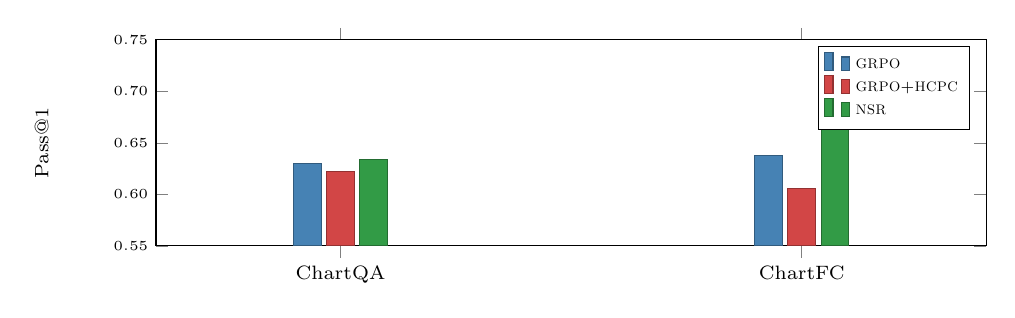
\begin{tikzpicture}
\scriptsize
\begin{axis}[
  ybar,
  bar width=10pt,
  width=\columnwidth,
  height=4.2cm,
  symbolic x coords={ChartQA, ChartFC},
  xtick=data,
  ylabel={Pass@1},
  ymin=0.55, ymax=0.75,
  ytick={0.55,0.60,0.65,0.70,0.75},
  y tick label style={
    /pgf/number format/fixed,
    /pgf/number format/fixed zerofill,
    /pgf/number format/precision=2,
    font=\tiny},
  x tick label style={font=\scriptsize},
  ylabel style={font=\scriptsize, at={(-0.12,0.5)}},
  legend style={at={(0.98,0.97)}, anchor=north east,
                legend columns=1, font=\tiny, inner sep=2pt,
                row sep=-1pt},
  legend cell align=left,
  enlarge x limits=0.4,
]
\addplot[fill=grpocol, draw=grpocol!70!black]
  coordinates {(ChartQA,0.630) (ChartFC,0.638)};
\addplot[fill=hcpccol, draw=hcpccol!70!black]
  coordinates {(ChartQA,0.622) (ChartFC,0.606)};
\addplot[fill=nsrcol,  draw=nsrcol!70!black]
  coordinates {(ChartQA,0.634) (ChartFC,0.708)};
\legend{\grpo, \grpo{}+\hcpc, \nsr}
\end{axis}
\end{tikzpicture}
\vspace{-0.25cm}
\caption{Pass@1 comparison on ChartQA (in-domain) and ChartFC (OOD).
  \nsr{}'s advantage grows from $+$0.4~pp in-domain to $+$7.0~pp OOD,
  consistent with its distribution-preserving update rule.}
\label{fig:p1}
\vspace{-0.3cm}
\end{figure}

\paragraph{RQ3: Reasoning diversity.}
$D_\text{reason}$ is nearly constant across all methods: 0.040 (base),
0.058 (\grpo), 0.052 (\hcpc), 0.056 (\nsr).
The explicit diversity reward in \hcpc{} does not increase $D_\text{reason}$
relative to \grpo---it marginally decreases it.
A 3B-parameter model generates reasoning traces that are highly similar in
pairwise sentence-embedding space regardless of the training signal; the
per-rollout uniqueness $u_k \approx 0.06$ is near-constant across correct rollouts,
making $w_r u_k$ an additive noise term rather than a differentiating gradient.

\paragraph{RQ4: Per-type breakdown.}
As shown in Table~\ref{tab:bytype}, \hcpc{}'s strongest gains appear on boolean
($+$3.5~pp over \grpo) and list-type questions, where binary answer spaces and
unambiguous rewards make the cross-rollout consistency signal most effective.
\grpo{} dominates on string questions (0.711) where positive reinforcement of
correct lookups is sufficient.
\nsr{} closely trails \grpo{} on numeric questions (0.624 vs.\ 0.631) despite
providing no positive gradient.

\paragraph{RQ5: Stage failure analysis.}
As shown in Table~\ref{tab:stage}, on ChartQA, conditional accuracy given correct
table extraction is highest for \hcpc{} (0.636, $+$1.4~pp over \grpo), confirming
that the table-consistency signal genuinely improves reasoning quality for rollouts
that extract data correctly.
On ChartFC, however, \grpo{}+\hcpc{} format compliance collapses to 0.560 while
both \grpo{} and \nsr{} maintain $\ge$0.991.

The root cause is that ChartFC provides no ground-truth tables ($\mathcal{T}^* = \varnothing$),
so the table-similarity gate in Eq.~(\ref{eq:filter}) is skipped entirely.
Without the format gate, a bare \texttt{Yes} response can enter $\mathcal{F}$
through the answer gate alone, receiving the cross-rollout bonus.
The model learns that format-free responses are acceptable on fact-checking
inputs---a reward-pool contamination effect that rapidly degrades format compliance.
Enforcing parse-success and table-schema checks before any rollout enters
$\mathcal{F}$ corrects this; the results above were produced before this fix was
applied, exposing the failure mode empirically.

\begin{table}[t]
  \centering
  \small
  \resizebox{\columnwidth}{!}{%
  \begin{tabular}{l|rrr}
    \toprule
    \textbf{Type} & \grpo & {+\hcpc} & \nsr \\
    \midrule
    Numeric  \small($n{=}290$)  & 0.631 & 0.614          & 0.624 \\
    Boolean  \small($n{=}87$)   & 0.586 & \textbf{0.621} & 0.598 \\
    String   \small($n{=}114$)  & \textbf{0.711} & 0.649 & 0.693 \\
    List     \small($n{=}9$)    & 0.000 & \textbf{0.556} & \textbf{0.556} \\
    \bottomrule
  \end{tabular}}
  \vspace{-0.15cm}
  \caption{ChartQA pass@1 by answer type.}
  \label{tab:bytype}
  \vspace{-0.2cm}
\end{table}

\begin{table}[t]
  \centering
  \small
  \resizebox{\columnwidth}{!}{%
  \begin{tabular}{l|rrrr}
    \toprule
    & \textbf{Fmt} & \textbf{Tbl} & \textbf{Ans} & \textbf{P(a$|$t)} \\
    \midrule
    \multicolumn{5}{l}{\small\textit{ChartQA}} \\[1pt]
    \grpo       & 0.962 & 0.953 & 0.609 & 0.622 \\
    +\hcpc      & 0.975 & 0.957 & 0.629 & \textbf{0.636} \\
    \nsr        & 0.970 & 0.960 & 0.622 & 0.632 \\
    \midrule
    \multicolumn{5}{l}{\small\textit{ChartFC}} \\[1pt]
    \grpo       & 0.991 & 0.996 & 0.661 & {--} \\
    +\hcpc      & 0.560 & 0.861 & 0.625 & {--} \\
    \nsr        & 0.991 & 0.997 & 0.687 & {--} \\
    \bottomrule
  \end{tabular}}
  \vspace{-0.15cm}
  \caption{Per-stage pass rate at rollout level.
    Fmt = format compliance; Tbl = valid JSON table;
    Ans = correct answer; P(a$|$t) = conditional accuracy given valid table.}
  \label{tab:stage}
  \vspace{-0.2cm}
\end{table}

%==================================================================
\section{Conclusion}

We proposed \hcpc-\rlvr, a cross-rollout reward applied to fully-correct rollouts
that incentivizes type and table consistency alongside per-rollout reasoning
diversity, and conducted the first evaluation of \nsr{} on a VLM.
\nsr{} is the strongest method on pass@1 across both benchmarks, with a 7.0~pp
OOD advantage on ChartFC attributable to preserving a broad distribution over
valid solution strategies.
\hcpc{} achieves the best pass@4 and improves boolean accuracy, but is constrained
by three failure modes: reasoning diversity is structurally capped at 3B-parameter
scale; the cross-rollout bonus is asymmetrically concentrated on easy samples where
$|\mathcal{F}| \ge 2$; and missing format gates allow reward-pool contamination on
fact-checking inputs.
For practitioners: (1)~always enforce a format gate before rollouts enter
$\mathcal{F}$; (2)~drop $D_\text{reason}$ at scales below 7B where diversity is
structurally capped; (3)~isolate the $C_\text{table}$ signal as the most reliable
\hcpc{} component at 3B scale.

%==================================================================
\section*{Acknowledgments}
We thank Syed Rifat Raiyan, Dr.\ Hasan Mahmud, and Dr.\ Md.\ Kamrul Hasan for
guidance and feedback throughout this work.

%==================================================================
\section*{Limitations}
(i)~All experiments use Qwen2.5-VL-3B-Instruct; the $D_\text{reason}$ saturation
and asymmetric signal effects may differ at larger scales ($\ge$7B parameters).
(ii)~Resource constraints limited rollout count to $K = 4$, below the intended
$K = 8$ for reliable cross-rollout estimates, potentially underestimating \hcpc{}'s
effectiveness.
(iii)~Training and evaluation use 1{,}000 and 500-sample subsets; results should
be confirmed on full splits and additional OOD benchmarks such as PlotQA~\citep{plotqa}
and ChartX~\citep{chartx2024}.

%==================================================================
\section*{Ethics Statement}
All datasets used in this work are publicly available.
No sensitive personal data is involved in chart question answering.
Experiments were conducted objectively with no intentional bias in data
selection or evaluation.

%==================================================================
\bibliography{paper}

\end{document}
